% 48-20(48쪽) — 세 함수 $f(x)=\log_a x$, $g(x)=\log_b x$, $h(x)=-\log_a x$ 의 그래프와 직선 $x=4$ 의 교점 A·B·C(원문 「오른쪽 그림」). 스캔 화질이 낮아 TikZ 로 다시 그림.
% 라벨은 원문에 있는 것만 — 세 곡선 이름, 점 A·B·C, 눈금 1·4 와 직선 $x=4$, 원점 O. $h(b)$(답)는 그림에서 읽히지 않게 적지 않는다.
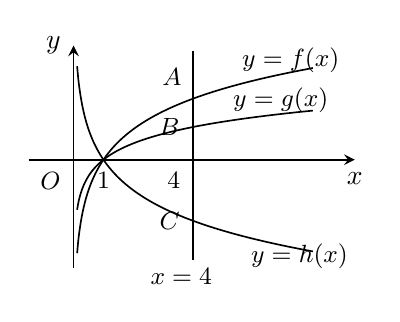
\begin{tikzpicture}[line width=0.6pt, x=0.38cm, y=0.50cm, >=stealth]
  \draw[->, line width=0.7pt] (-1.5,0) -- (9.4,0) node[below=1pt] {$x$};
  \draw[->, line width=0.7pt] (0,-2.75) -- (0,2.9) node[left=1pt] {$y$};
  \draw[line width=0.7pt] (4,-2.55) -- (4,2.75);
  \draw[domain=0.12:8.0, samples=180, smooth] plot (\x, {1.12*ln(\x)});
  \draw[domain=0.12:8.0, samples=180, smooth] plot (\x, {0.60*ln(\x)});
  \draw[domain=0.12:8.0, samples=180, smooth] plot (\x, {-1.12*ln(\x)});
  \node[font=\small, anchor=south east] at (3.95,1.62) {$\pt{A}$};
  \node[font=\small, anchor=east] at (3.88,0.84) {$\pt{B}$};
  \node[font=\small, anchor=east] at (3.88,-1.55) {$\pt{C}$};
  \node[font=\small, anchor=north] at (1.0,-0.08) {$1$};
  \node[font=\small, anchor=north east] at (3.90,-0.08) {$4$};
  \node[font=\small, anchor=north east] at (-0.10,-0.08) {$\pt{O}$};
  \node[font=\small, anchor=north] at (3.6,-2.50) {$x=4$};
  \node[font=\small, anchor=west] at (5.3,2.52) {$y=f(x)$};
  \node[font=\small, anchor=west] at (5.0,1.50) {$y=g(x)$};
  \node[font=\small, anchor=west] at (5.6,-2.45) {$y=h(x)$};
\end{tikzpicture}
